\documentclass{if-beamer}

% --------------------------------------------------- %
%                  Presentation info	              %
% --------------------------------------------------- %
\title[Pesquisa Operacional]{\textbf{Pesquisa Operacional I}}
\subtitle{Programação Linear}
\author[Haron Calegari Fanticelli]{\large \negrito{Haron Calegari Fanticelli}}
\institute[CEFET/RJ]{
    \small \textit{Centro Federal de Educação Tecnológica Celso Suckow da Fonseca} \\
    \textit{Uned Itaguaí}
}
\date{\today}
\logo{

\includegraphics[scale=.1, clip]{ufpr.png}
}
\subject{Presentation subject} % metadata
%trim={<left> <lower> <right> <upper>}
\graphicspath{{figuras/}}
% --------------------------------------------------- %
%                    Title + Schedule                 %
% --------------------------------------------------- %

\begin{document}

\begin{frame}
  \titlepage
\end{frame}

\begin{frame}{Programação}
  \tableofcontents
\end{frame}

% --------------------------------------------------- %
%                      Presentation                   %
% --------------------------------------------------- %

%%%%%%%%%%%%%%%%%%%%%%%%%%%%%%%%%%%%%%%%%%%%%%%%%%%%%%%%%%%%%

\section{Recapitulação}

%%%%%%%%%%%%%%%%%%%%%%%%%%%%%%%%%%%%%%%%%%%%%%%%%%%%%%%%%%%%%

\subsection{Forma-padrão}
\begin{frame}{Modelo de Otimização}

\begin{minipage}{.49\textwidth}

\begin{itemize}
    \item Forma-padrão (HILLIER, 2010):
\end{itemize}
\begin{align*}
\begin{matrix}
    \textbf{Maximizar:} & f(\mathbf{x}) & & \\
    \textbf{Sujeito a:} & A\mathbf{x} & = & \mathbf{b} \\
    \textbf{e:} & \mathbf{x} & \geq & 0
\end{matrix}    
\end{align*}

%em que $\mathbf{x} = (x_1, x_2, \dots,x_n)^t$, $\mathbf{b} = (b_1, b_2, \dots, b_n)^t$, $f(\mathbf{x})$ é a função que pretendemos maximizar, $A_{m \times n}$ é a matriz de coeficientes, $m$ a quantidade de restrições e $n$ a quantidade de variáveis.

\end{minipage}
\begin{minipage}{.49\textwidth}

\end{minipage}

\end{frame}

%%%%%%%%%%%%%%%%%%%%%%%%%%%%%%%%%%%%%%%%%%%%%%%%%%%%%%%%%%%%%

\begin{frame}{Modelo de Otimização}

\begin{minipage}{.49\textwidth}

\begin{itemize}
    \item Forma-padrão (HILLIER, 2010):
\end{itemize}
\begin{align*}
\begin{matrix}
    \textbf{Maximizar:} & f(\mathbf{x}) & & \\
    \textbf{Sujeito a:} & A\mathbf{x} & = & \mathbf{b} \\
    \textbf{e:} & \mathbf{x} & \geq & 0
\end{matrix}    
\end{align*}

\vspace{.8cm}

\begin{itemize}
    \item Exemplo:
\end{itemize}
\begin{align*}
\begin{matrix}
    \textbf{Maximizar:} & Z & = & 3x_1 & + & 5x_2 \\
    \textbf{Sujeito a:} &  x_1 &   &      & \leq & 4  \\
                        &      &   & 2x_2 & \leq & 12 \\
                        & 3x_1 & + & 2x_2 & \leq & 18 \\
    \textbf{e:}         &      & \mathbf{x} & \geq & 0 & 
\end{matrix}
\end{align*}

\end{minipage}
\begin{minipage}{.49\textwidth}

\end{minipage}

\end{frame}

%%%%%%%%%%%%%%%%%%%%%%%%%%%%%%%%%%%%%%%%%%%%%%%%%%%%%%%%%%%%%

\subsection{Método do Gráfico}
\begin{frame}{Modelo de Otimização}

\begin{minipage}{.49\textwidth}

\begin{itemize}
    \item Forma-padrão (HILLIER, 2010):
\end{itemize}
\begin{align*}
\begin{matrix}
    \textbf{Maximizar:} & f(\mathbf{x}) & & \\
    \textbf{Sujeito a:} & A\mathbf{x} & = & \mathbf{b} \\
    \textbf{e:} & \mathbf{x} & \geq & 0
\end{matrix}    
\end{align*}

\vspace{.8cm}

\begin{itemize}
    \item Exemplo:
\end{itemize}
\begin{align*}
\begin{matrix}
    \textbf{Maximizar:} & Z & = & 3x_1 & + & 5x_2 \\
    \textbf{Sujeito a:} &  x_1 &   &      & \leq & 4  \\
                        &      &   & 2x_2 & \leq & 12 \\
                        & 3x_1 & + & 2x_2 & \leq & 18 \\
    \textbf{e:}         &      & \mathbf{x} & \geq & 0 & 
\end{matrix}
\end{align*}

\end{minipage}
\begin{minipage}{.49\textwidth}

\begin{figure}
    \centering
    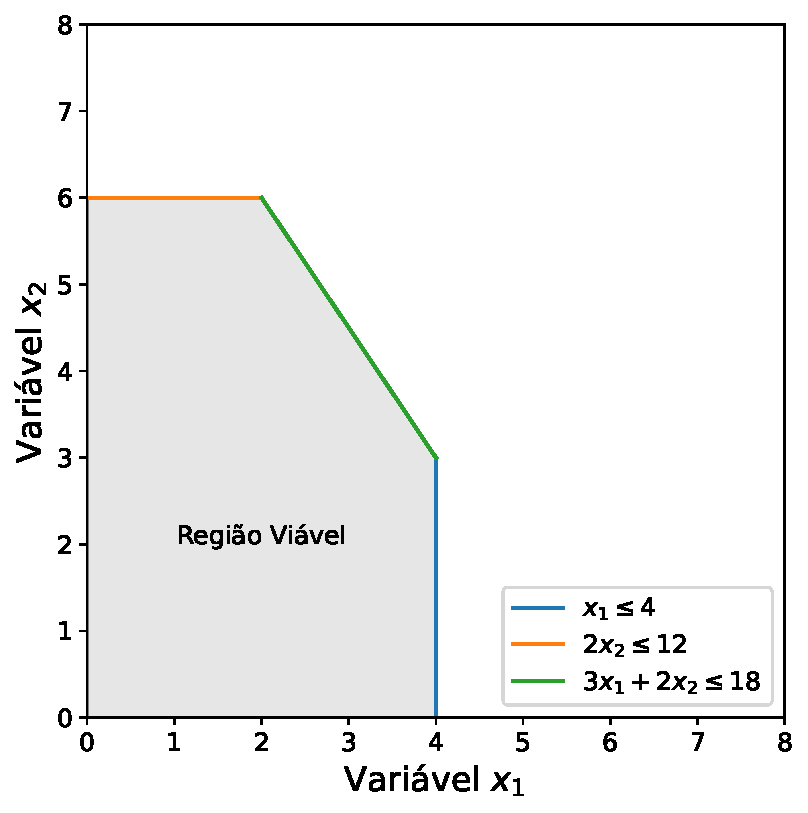
\includegraphics[scale=.45]{figuras/fig_wyndor.pdf}
    \caption{Gráfico de Região Viável}
\end{figure}

\end{minipage}

\end{frame}

%%%%%%%%%%%%%%%%%%%%%%%%%%%%%%%%%%%%%%%%%%%%%%%%%%%%%%%%%%%%%

\begin{frame}{Modelo de Otimização}

\begin{minipage}{.49\textwidth}

\begin{itemize}
    \item Forma-padrão (HILLIER, 2010):
\end{itemize}
\begin{align*}
\begin{matrix}
    \textbf{Maximizar:} & f(\mathbf{x}) & & \\
    \textbf{Sujeito a:} & A\mathbf{x} & = & \mathbf{b} \\
    \textbf{e:} & \mathbf{x} & \geq & 0
\end{matrix}    
\end{align*}

\vspace{.8cm}

\begin{itemize}
    \item Exemplo:
\end{itemize}
\begin{align*}
\begin{matrix}
    \textbf{Maximizar:} & Z & = & 3x_1 & + & 5x_2 \\
    \textbf{Sujeito a:} &  x_1 &   &      & \leq & 4  \\
                        &      &   & 2x_2 & \leq & 12 \\
                        & 3x_1 & + & 2x_2 & \leq & 18 \\
    \textbf{e:}         &      & \mathbf{x} & \geq & 0 & 
\end{matrix}    
\end{align*}

\end{minipage}
\begin{minipage}{.49\textwidth}

\begin{figure}
    \centering
    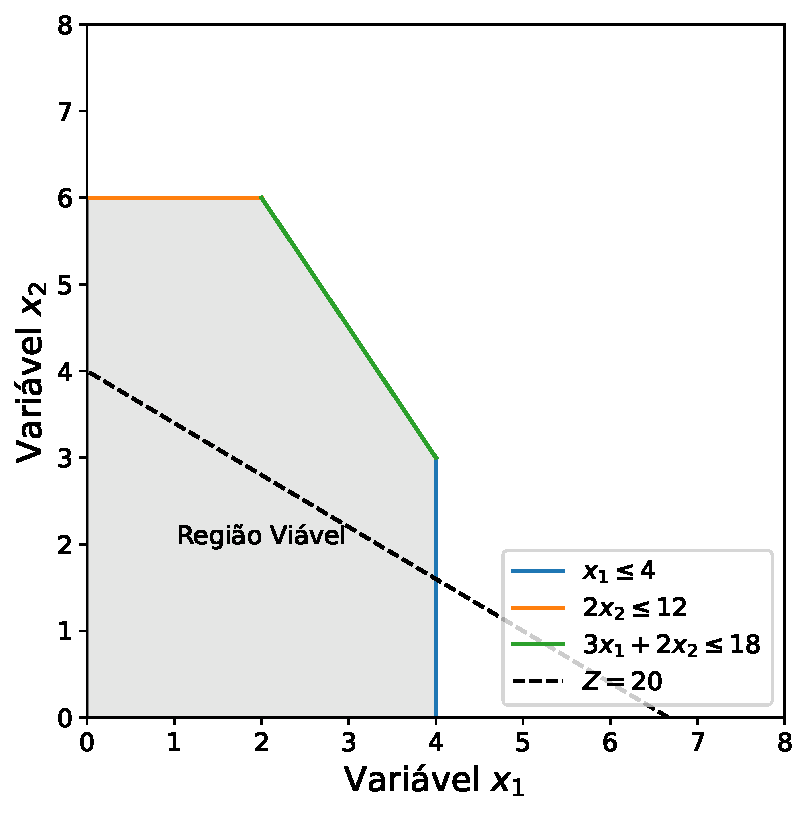
\includegraphics[scale=.45]{figuras/fig_wyndor_Z.pdf}
    \caption{Gráfico de Região Viável}
\end{figure}

\end{minipage}

\end{frame}

%%%%%%%%%%%%%%%%%%%%%%%%%%%%%%%%%%%%%%%%%%%%%%%%%%%%%%%%%%%%%

\section{O Método Simplex}

%%%%%%%%%%%%%%%%%%%%%%%%%%%%%%%%%%%%%%%%%%%%%%%%%%%%%%%%%%%%%

\subsection{Introdução}
\begin{frame}{Introdução}
\begin{itemize}
    \item Proposto em 1947 por George B. Dantzig;
    \item 2000: Reconhecido como um dos 10 algoritmos mais importantes do século 20 (IEEE);
\end{itemize}
\begin{figure}
    \centering
    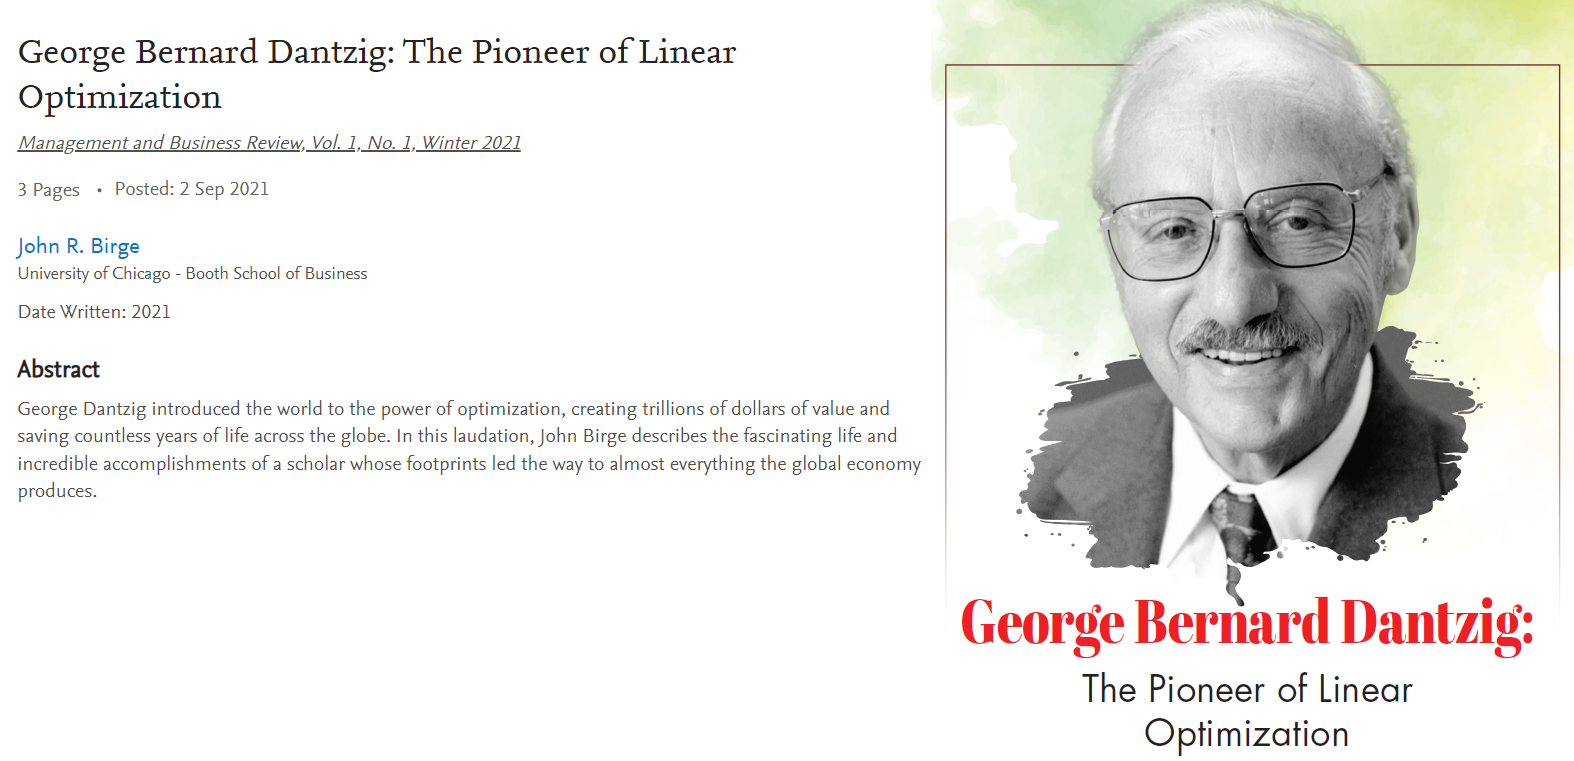
\includegraphics[scale=.3]{figuras/artigo_dantzig.png}
\end{figure}

\end{frame}

%%%%%%%%%%%%%%%%%%%%%%%%%%%%%%%%%%%%%%%%%%%%%%%%%%%%%%%%%%%%%

\subsection{Forma Tabular (Algoritmo)}
\begin{frame}{Forma Tabular do Simplex}

\begin{itemize}
    \item \negrito{Config 01:} Colocar o modelo na forma padrão;
\end{itemize}

\begin{align*}
\begin{matrix}
    \textbf{Maximizar:} & Z & = & 3x_1 & + & 5x_2 & & \\
    \textbf{Sujeito a:} & & &  x_1 &   &      & \leq & 4  \\
                        & & &      &   & 2x_2 & \leq & 12 \\
                        & & & 3x_1 & + & 2x_2 & \leq & 18 \\
    \textbf{e:}         & & &      & \mathbf{x} & \geq & 0 & 
\end{matrix}    
\end{align*}

\end{frame}

%%%%%%%%%%%%%%%%%%%%%%%%%%%%%%%%%%%%%%%%%%%%%%%%%%%%%%%%%%%%%

\begin{frame}{Forma Tabular do Simplex}

\begin{itemize}
    \item \negrito{Config 01:} Colocar o modelo na forma padrão (Variáveis de Folga);
\end{itemize}

\begin{align*}
\begin{matrix}
    \textbf{Maximizar:} & Z = 3x_1 + 5x_2 + 0f_1 + 0f_2 + 0f_3 \\
    \textbf{Sujeito a:} & 
\end{matrix}
\end{align*}
\vspace{-.6cm}
\begin{align*}
\begin{matrix}
     x_1 &        & + f_1 &       &       & = & 4  \\ 
         &   2x_2 &       & + f_2 &       & = & 12 \\
    3x_1 & + 2x_2 &       &       & + f_3 & = & 18
\end{matrix}
\end{align*}
\begin{align*}
\begin{matrix}
    \textbf{e:} & \mathbf{x} \geq 0 & \mathbf{f} \geq 0
\end{matrix}
\end{align*}

\end{frame}

%%%%%%%%%%%%%%%%%%%%%%%%%%%%%%%%%%%%%%%%%%%%%%%%%%%%%%%%%%%%%

\begin{frame}{Forma Tabular do Simplex}

\begin{itemize}
    \item \negrito{Config 01:} Colocar o modelo na forma padrão (Variáveis de Folga);
    \item \negrito{Config 02:} Colocar a função objetivo Z = 0;
\end{itemize}

\begin{align*}
\begin{matrix}
    \textbf{Maximizar:} & Z - 3x_1 - 5x_2 - 0f_1 - 0f_2 - 0f_3 = 0 \\
    \textbf{Sujeito a:} & 
\end{matrix}
\end{align*}
\vspace{-.6cm}
\begin{align*}
\begin{matrix}
     x_1 &        & + f_1 &       &       & = & 4  \\ 
         &   2x_2 &       & + f_2 &       & = & 12 \\
    3x_1 & + 2x_2 &       &       & + f_3 & = & 18
\end{matrix}
\end{align*}
\begin{align*}
\begin{matrix}
    \textbf{e:} & \mathbf{x} \geq 0 & \mathbf{f} \geq 0
\end{matrix}
\end{align*}

\end{frame}

%%%%%%%%%%%%%%%%%%%%%%%%%%%%%%%%%%%%%%%%%%%%%%%%%%%%%%%%%%%%%

\begin{frame}{Forma Tabular do Simplex}

\begin{itemize}
    \item \negrito{Config 01:} Colocar o modelo na forma padrão (Variáveis de Folga);
    \item \negrito{Config 02:} Colocar a função objetivo Z = 0;
    \item \negrito{Config 03:} Tabular as variáveis;
    \item \negrito{Config 04:} Variáveis Básicas = 0 / Solução Inicial na Origem;
\end{itemize}

\begin{table}
    \centering
    \begin{tabular}{c|ccccccc}
    \hline
    VB    & $Z$ & $x_1$ & $x_2$ & $f_1$ & $f_2$ & $f_3$ & $=$  \\
    \hline
    $Z$   & 1   & -3    & -5    & 0     & 0     & 0     & 0    \\
    $f_1$ & 0   & 1     & 0     & 1     & 0     & 0     & 4    \\
    $f_2$ & 0   & 0     & 2     & 0     & 1     & 0     & 12   \\
    $f_3$ & 0   & 3     & 2     & 0     & 0     & 1     & 18   \\
    \hline
    \end{tabular}
\end{table}

\end{frame}

%%%%%%%%%%%%%%%%%%%%%%%%%%%%%%%%%%%%%%%%%%%%%%%%%%%%%%%%%%%%%

\begin{frame}{Forma Tabular do Simplex}

\negrito{1ª Iteração}
\begin{itemize}
    \item \negrito{Passo 01:} Coluna Pivô (Objetivo) - Escolher Menor valor (negativo);
\end{itemize}

\begin{table}
    \centering
    \begin{tabular}{c|ccccccc}
    \hline
    VB    & $Z$ & $x_1$ & $x_2$ & $f_1$ & $f_2$ & $f_3$ & $=$  \\
    \hline
    $Z$   & 1   & -3    & -5    & 0     & 0     & 0     & 0    \\
    $f_1$ & 0   & 1     & 0     & 1     & 0     & 0     & 4    \\
    $f_2$ & 0   & 0     & 2     & 0     & 1     & 0     & 12   \\
    $f_3$ & 0   & 3     & 2     & 0     & 0     & 1     & 18   \\
    \hline
    \end{tabular}
\end{table}

\end{frame}

%%%%%%%%%%%%%%%%%%%%%%%%%%%%%%%%%%%%%%%%%%%%%%%%%%%%%%%%%%%%%

\begin{frame}{Forma Tabular do Simplex}

\negrito{1ª Iteração}
\begin{itemize}
    \item \negrito{Passo 01:} Coluna Pivô (Objetivo) - Escolher Menor valor (negativo);
    \item \negrito{Passo 02:} Linha Pivô (Restrições) - Escolher Menor Razão (positivo);
\end{itemize}

\begin{table}
    \centering
    \begin{tabular}{c|cc >{\columncolor[HTML]{CBCEFB}}c cccc}
    \hline
    VB    & $Z$ & $x_1$ & $x_2$ & $f_1$ & $f_2$ & $f_3$ & $=$  \\
    \hline
    $Z$   & 1   & -3    & -5    & 0     & 0     & 0     & 0    \\
    $f_1$ & 0   & 1     & 0     & 1     & 0     & 0     & 4    \\
    $f_2$ & 0   & 0     & 2     & 0     & 1     & 0     & 12   \\
    $f_3$ & 0   & 3     & 2     & 0     & 0     & 1     & 18   \\
    \hline
    \end{tabular}
\end{table}

\end{frame}

%%%%%%%%%%%%%%%%%%%%%%%%%%%%%%%%%%%%%%%%%%%%%%%%%%%%%%%%%%%%%

\begin{frame}{Forma Tabular do Simplex}

\textcolor{airforceblue}{\textbf{1ª Iteração}}
\begin{itemize}
    \item \negrito{Passo 01:} Coluna Pivô (Objetivo) - Escolher Menor valor (negativo);
    \item \negrito{Passo 02:} Linha Pivô (Restrições) - Escolher Menor Razão (positivo);
    \item \negrito{Passo 03:} Fazer a troca de variáveis - Operações Elementares;
\end{itemize}

\begin{table}
    \centering
    \begin{tabular}{cc|cc >{\columncolor[HTML]{CBCEFB}}c cccc}
    & & & & $\downarrow$ & & & & \\
    \hline
    & VB    & $Z$ & $x_1$ & $x_2$ & $f_1$ & $f_2$ & $f_3$ & $=$  \\
    \hline
    & $Z$   & 1   & -3    & -5    & 0     & 0     & 0     & 0    \\
    & $f_1$ & 0   & 1     & 0     & 1     & 0     & 0     & 4    \\
    \rowcolor[HTML]{CBCEFB}
    $\leftarrow$ & $f_2$ & 0   & 0     & 2     & 0     & 1     & 0     & 12   \\
    & $f_3$ & 0   & 3     & 2     & 0     & 0     & 1     & 18   \\
    \hline
    \end{tabular}
\end{table}

\end{frame}

%%%%%%%%%%%%%%%%%%%%%%%%%%%%%%%%%%%%%%%%%%%%%%%%%%%%%%%%%%%%%

\begin{frame}{Forma Tabular do Simplex}

\negrito{1ª Iteração}
\begin{itemize}
    \item \negrito{Passo 01:} Coluna Pivô (Objetivo) - Escolher Menor valor (negativo);
    \item \negrito{Passo 02:} Linha Pivô (Restrições) - Escolher Menor Razão (positivo);
    \item \negrito{Passo 03:} Fazer a troca de variáveis - Operações Elementares;
    \item \negrito{Passo 04:} Critério de Parada - Função objetivo não possuir valores negativos;
\end{itemize}

\begin{table}
    \centering
    \begin{tabular}{c|ccccccc}
    \hline
    VB    & $Z$ & $x_1$ & $x_2$ & $f_1$ & $f_2$ & $f_3$ & $=$  \\
    \hline
    $Z$   & 1   & -3    & 0     & 0     & 2.5   & 0     & 30   \\
    $f_1$ & 0   & 1     & 0     & 1     & 0     & 0     & 4    \\
    $x_2$ & 0   & 0     & 1     & 0     & 0.5   & 0     & 6    \\
    $f_3$ & 0   & 3     & 0     & 0     & -1    & 1     & 6    \\
    \hline
    \end{tabular}
\end{table}

\end{frame}

%%%%%%%%%%%%%%%%%%%%%%%%%%%%%%%%%%%%%%%%%%%%%%%%%%%%%%%%%%%%%

\subsection{Exemplo}
\begin{frame}{Forma Tabular do Simplex}

\negrito{2ª Iteração}
\begin{itemize}
    \item \negrito{Passo 01:} Coluna Pivô (Objetivo) - Escolher Menor valor (negativo);
    \item \negrito{Passo 02:} Linha Pivô (Restrições) - Escolher Menor Razão (positivo);
    \item \negrito{Passo 03:} Fazer a troca de variáveis - Operações Elementares;
    \item \negrito{Passo 04:} Critério de Parada - Função objetivo não possuir valores negativos;
\end{itemize}

\begin{table}
    \centering
    \begin{tabular}{c|ccccccc}
    \hline
    VB    & $Z$ & $x_1$ & $x_2$ & $f_1$ & $f_2$ & $f_3$ & $=$  \\
    \hline
    $Z$   & 1   & 0     & 0     & 0     & 1.5   & 1     & 36   \\
    $f_1$ & 0   & 0     & 0     & 1     & 0.33  & -0.33 & 2    \\
    $x_2$ & 0   & 0     & 1     & 0     & 0.5   & 0     & 6    \\
    $x_1$ & 0   & 1     & 0     & 0     & -0.33 & 0.33  & 2    \\
    \hline
    \end{tabular}
\end{table}

\end{frame}

%%%%%%%%%%%%%%%%%%%%%%%%%%%%%%%%%%%%%%%%%%%%%%%%%%%%%%%%%%%%%

\begin{frame}{Forma Tabular do Simplex}

\negrito{2ª Iteração}
\begin{itemize}
    \item \negrito{Passo 01:} Coluna Pivô (Objetivo) - Escolher Menor valor (negativo);
    \item \negrito{Passo 02:} Linha Pivô (Restrições) - Escolher Menor Razão (positivo);
    \item \negrito{Passo 03:} Fazer a troca de variáveis - Operações Elementares;
    \item \negrito{Passo 04:} Critério de Parada - Função objetivo não possuir valores negativos;
\end{itemize}

\begin{table}
    \centering
    \begin{tabular}{c|ccccccc}
    \hline
    VB    & $Z$ & $x_1$ & $x_2$ & $f_1$ & $f_2$ & $f_3$ & $=$  \\
    \hline
    $Z$   & 1   & 0     & 0     & 0     & 1.5   & 1     & 36   \\
    $f_1$ & 0   & 0     & 0     & 1     & 0.33  & -0.33 & 2    \\
    \rowcolor[HTML]{CBCEFB}
    $x_2$ & 0   & 0     & 1     & 0     & 0.5   & 0     & 6    \\
    \rowcolor[HTML]{CBCEFB}
    $x_1$ & 0   & 1     & 0     & 0     & -0.33 & 0.33  & 2    \\
    \hline
    \end{tabular}
\end{table}

\negrito{Solução Ótima:} $\mathbf{x} = (2,6)$ e $Z = 36$

\end{frame}

%%%%%%%%%%%%%%%%%%%%%%%%%%%%%%%%%%%%%%%%%%%%%%%%%%%%%%%%%%%%%

\section{Atividade de Aprendizagem}

%%%%%%%%%%%%%%%%%%%%%%%%%%%%%%%%%%%%%%%%%%%%%%%%%%%%%%%%%%%%%

\begin{frame}{Atividade de Aprendizagem}

\begin{minipage}[t]{.49\textwidth}
\begin{itemize}
\justifying
    \item \textbf{(1)} Um certo modelo de programação linear envolvendo duas atividades possui a região de soluções viáveis indicada a seguir.

    \begin{figure}
        \centering
        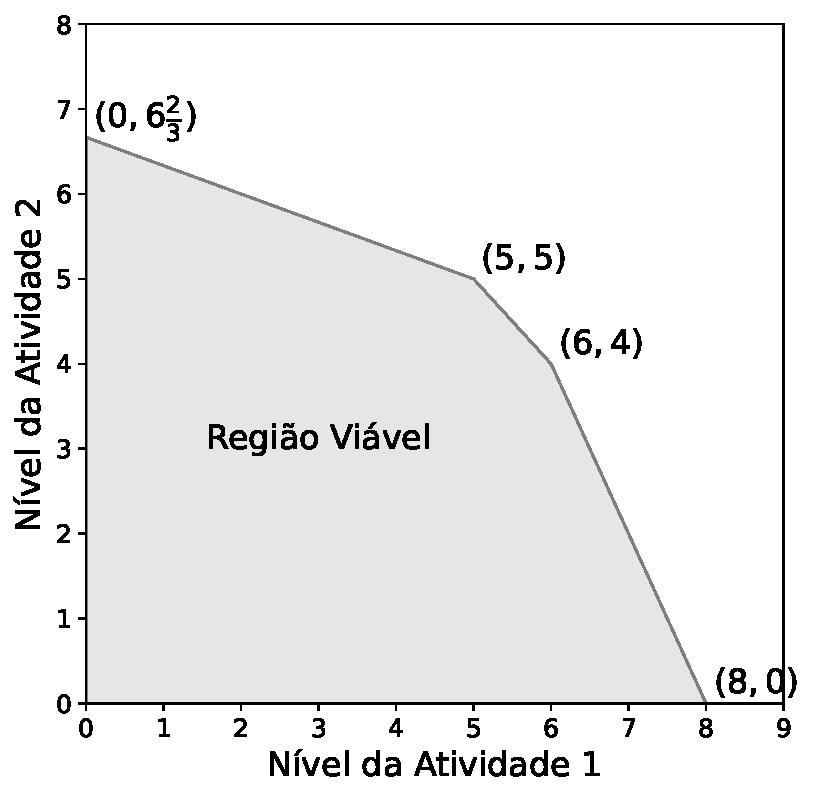
\includegraphics[scale=0.35]{figuras/exerc_4.1-3.pdf}
    \end{figure}
\end{itemize}
\end{minipage}\hfill
\begin{minipage}[t]{.49\textwidth}
\justifying
O objetivo é maximizar o lucro total das duas atividades. O lucro unitário para a atividade 1 é de US\$ 1.000 e o lucro unitário para a atividade 2 é de US\$ 2.000.
\begin{itemize}
    \justifying
    \item \textbf{(a)} Calcule o lucro total para cada solução de pontos extremos. Use esta informação para encontrar uma solução ótima.
    \item \textbf{(b)} Use os conceitos de solução do Método Simplex para identificar a sequência de soluções que seriam examinados pelo método até chegar a solução ótima.
\end{itemize}
\end{minipage}

\end{frame}

%%%%%%%%%%%%%%%%%%%%%%%%%%%%%%%%%%%%%%%%%%%%%%%%%%%%%%%%%%%%%

\begin{frame}{Atividade de Aprendizagem}

\begin{itemize}
    \item \textbf{(2)} Pelo método simplex, passo a passo, solucione o problema a seguir:
    \begin{align*}
    \begin{matrix}
        \text{Maximizar} & Z = 4x_1 + 3x_2 + 6x_3 \\
        \text{Sujeito a} & 3x_1 + x_2 + 3x_3 \leq 30 \\
                         & 2x_1 + 2x_2 + 3x_3 \leq 40 \\
        \text{e}         & x_1 \geq 0 \text{, } x_2 \geq 0 \text{, } x_3 \geq 0
    \end{matrix}
    \end{align*}


    \item \textbf{(3)} Descreva graficamente o que o método simplex faz passo a passo para solucionar o problema a seguir:
    \begin{align*}
        \begin{matrix}
            \text{Maximizar} & Z = 2x_1 + 3x_2 \\
            \text{Sujeito a} & -3x_1 + x_2 \leq 1 \\
                             & 4x_1 + 2x_2 \leq 20 \\
                             & 4x_1 - x_2 \leq 10 \\
                             & -x_1 + 2x_2 \leq 5 \\
            \text{e}         & x_1 \geq 0 \text{, } x_2 \geq 0
        \end{matrix}
    \end{align*}
\end{itemize}

\end{frame}

%%%%%%%%%%%%%%%%%%%%%%%%%%%%%%%%%%%%%%%%%%%%%%%%%%%%%%%%%%%%%

\section{Referências e Próxima Aula}

%%%%%%%%%%%%%%%%%%%%%%%%%%%%%%%%%%%%%%%%%%%%%%%%%%%%%%%%%%%%%

\begin{frame}{Referências e Próxima Aula}

\begin{itemize}
    \item HILLIER, Frederick S.; LIEBERMAN, Gerald J. \textbf{Introdução à Pesquisa Operacional.} Porto Alegre: Bookman, 2010.
    \item TAHA, Hamdy A. \textbf{Pesquisa Operacional.} São Paulo: Pearson Prentice Hall, 2008.
\end{itemize}

\begin{block}{Próxima Aula}
    \begin{itemize}
        \item Empate para a Coluna Pivô (Variável Básica que Entra);
        \item Empate para a Linha Pivô (Variável Básica que Sai);
        \item Nenhuma Linha Pivô (Variável Básica que Sai) - Z Ilimitado;
        \item Soluções Ótimas Múltiplas.
    \end{itemize}
\end{block}

\end{frame}

%%%%%%%%%%%%%%%%%%%%%%%%%%%%%%%%%%%%%%%%%%%%%%%%%%%%%%%%%%%%%


%%%%%%%%%%%%%%%%%%%%%%%%%%%%%%%%%%%%%%%%%%%%%%%%%%%%%%%%%%%%%

{
\usebackgroundtemplate{
\includegraphics[width=\paperwidth]{obrigado.jpg}}
\begin{frame}[plain]
\end{frame}
}

\end{document}
